\section{Metodología de trabajo y herramientas} \label{cap:herram}

El trabajo realizado en el marco del TFM se ha llevado a cabo entre las 
instalaciones del edificio CITIC de la UGR y el laboratorio de sincronización 
de la empresa Seven Solutions (en el edificio CETIC de la UGR). Dada la 
naturaleza de este tipo de desarrollos se necesita una gran cantidad de 
material y herramientas que no suelen ser baratos, por lo que no siempre es 
fácil disponer de ellos. En resumen se han utilizado equipos \gls{wr} como el 
WR-LEN y el WR-ZEN, equipos de medición como osciloscopios y analizadores de 
\textit{Phase Noise}, multitud de fibras y demás material para formar redes WR, 
entre otras cosas.

La metodología de desarrollo ha seguido un modelo en cascada: primero se ha 
realizado una labor de análisis de la arquitectura actual en los nodos WR y de 
una implementación concreta de dicha arquitectura. Para ello se han realizado 
una serie de experimentos de caracterización que permiten extraer datos 
interesantes acerca de las limitaciones de la tecnología actual. Luego se 
introduce el nuevo desarrollo de una arquitectura basada en la familia de 
\gls{soc} Zynq-7000 de Xilinx y se llegan a varias 
conclusiones para aportar mejoras a la implementación actual. Por otra parte se 
analizar el aspecto \textit{hardware} relativo a la circuitería de reloj y se 
proponen una serie de mejoras en base a ese análisis y a una serie de 
resultados obtenidos tras una labor de caracterización. 

A continación se hace un listado del conjunto de herramientas utilizado durante 
el desarrollo de este TFM. En primer lugar mencionar los equipos WR utilizados:

\begin{itemize}
	\item Equipos \textbf{\gls{wrs}}, se utilizan como elementos intermedios de 
	la 
	red de 
	sincronización. Se caracterizan por incluir un gran número de interfaces 
	físicas para propagar la señal de sincronización de forma descendente.
	\begin{figure}
		\centering
		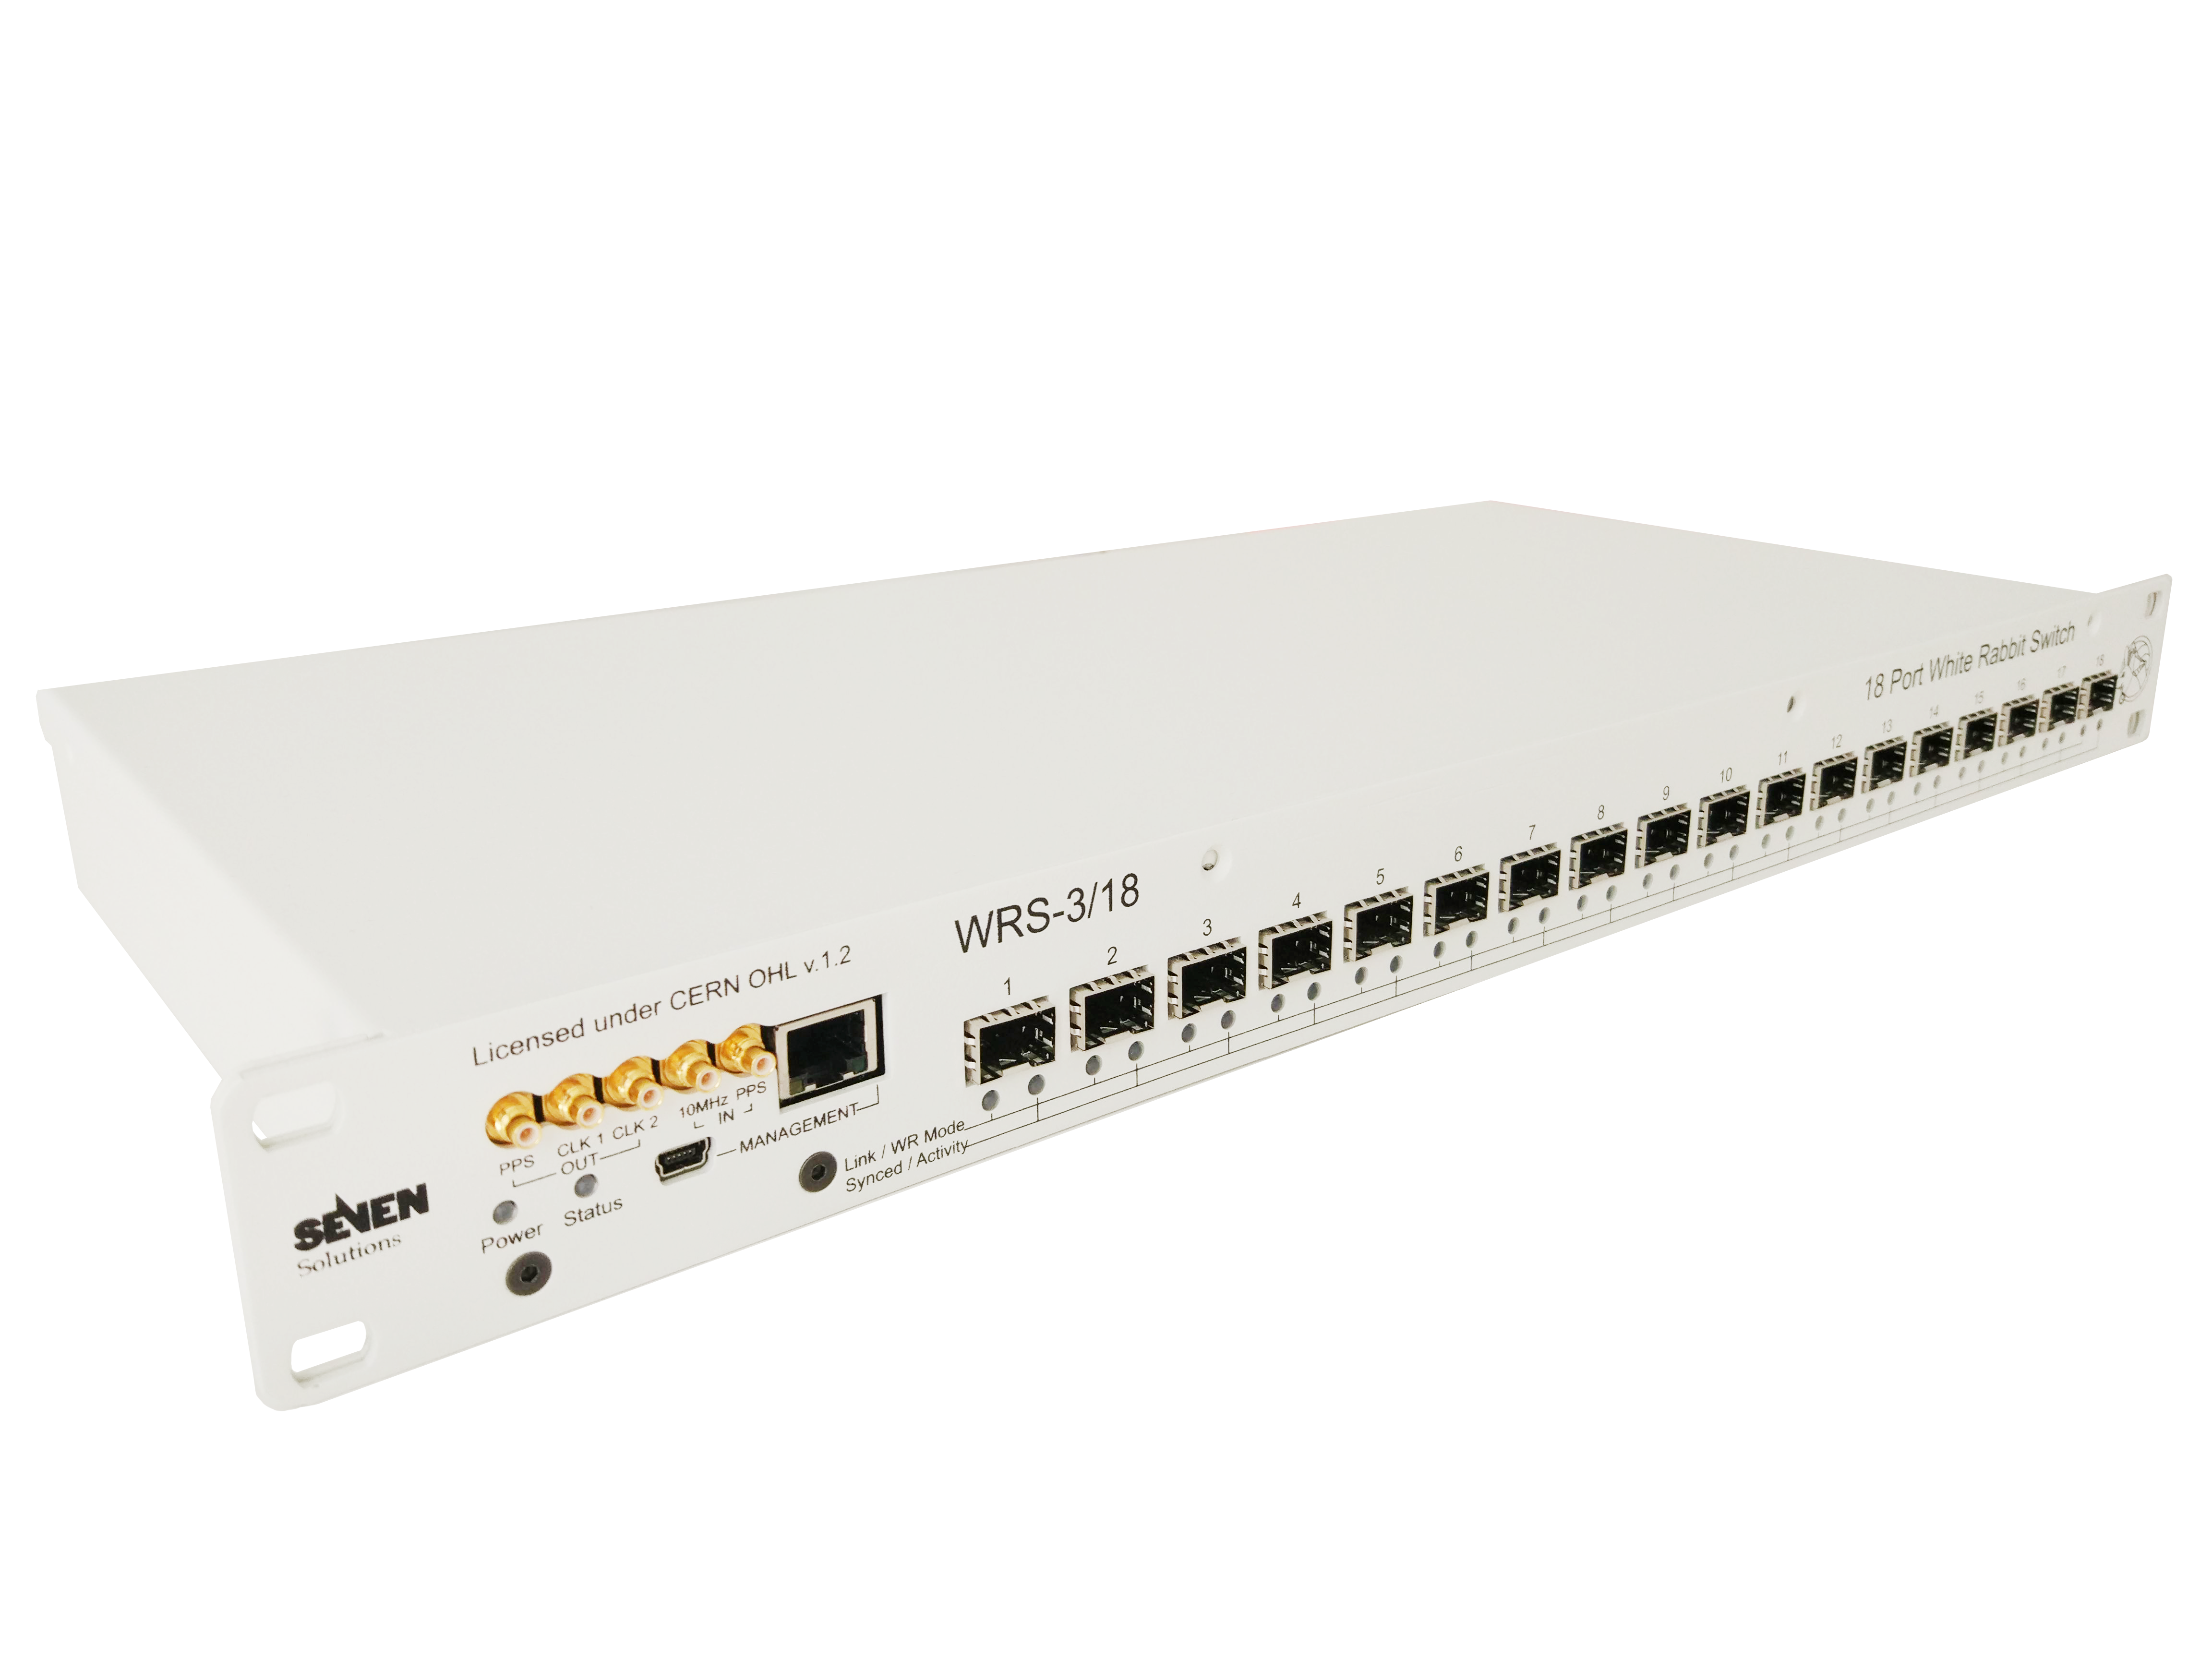
\includegraphics[width=0.4\linewidth]{imagenes/wrs}
		\caption[Imagen del White Rabbit Switch]{Imagen del White Rabbit Switch}
		\label{fig:wrs}
	\end{figure}
	 
	\item Equipos \textbf{WR-ZEN}. Este nuevo nodo incorpora la nueva 
	arquitectura basada en SoC-FPGA así como algunas de las nuevos elementos en 
	electrónica de generación de reloj de bajo ruido.
	\item Los equipos \textbf{WR-LEN} se han utilizado para pruebas con un gran 
	número de nodos debido a que su reducido tamaño y coste ha permitido 
	disponer de un gran número de estos. Su electrónica para el sistema de 
	relojes es similar a la incluida en el WRS.
\end{itemize}

Además han sido necesarios múltiples dispositivos de medida de alta resolución 
debido a las características tan exigentes del protocolo de sincronización WR:

\begin{itemize}
	\item \textbf{Osciloscopio} Tektronix DPO-7354.
	\item \textbf{Medidor de Phase Noise} Microsemi 3120A.
	\item \textbf{Frecuencímetro/Contador} Keysight 53230.
\end{itemize}

El material típico para realizar las conexiones de fibra o controlar los 
aparatos utilizados:

\begin{itemize}
	\item \textit{Transceivers} SFPs. Son los elementos que convierten las 
	señales eléctricas en lumínicas para transmitir la información por el 
	enlace de fibra óptica. En concreto se han utilizado los modelos SFP 
	AXGE-3454-0531 y AXGE-1254-0531 preparados para enlaces de hasta 10 km de 
	longitud.
	\item Convertidores SFP de 1000BaseLX (usado en WR) a 1000BaseT para poder 
	enviar tráfico y gestionar los nodos desde la interfaz Ethernet de un PC.
	\item Enlaces de fibra óptica de 1m y varias bobinas de 5km.
	\item Cables de RF para conectar las salidas de las tarjetas a los apartos 
	de medición. En concreto se han usado los conectores tipo SMA, SMC y BNC. 
	Es importante contar con cables que tengan un buen apantallamiento debido a 
	la sensibilidad de algunos aparatos utilizados al ruido electromagnético.
\end{itemize}

A parte de todos los componentes físicos, también han sido necesarias múltiples 
herramientas \textit{software}:

\begin{itemize}
	\item Sistema operativo GNU/Linux, enconcreto Ubuntu. Por suerte la mayoría 
	de herramientas de desarrollo para el ámbito de WR están preparadas para 
	este tipo de SO. Se necesitan versiones concretas (la LTS de turno) ya que 
	los proyectos suelen estar preparados para compilar bajo unas condiciones 
	de paquetes y versiones específicas. Intentar usar versiones más modernas u 
	otros SO requiere un gran manejo y una gran inversión de tiempo.
	
	\item Herramientas de control de versiones, como Git, para la gestión de 
	los repositorios disponibles en la web de \gls{ohwr} \cite{website:ohwr} 
	así como para los desarrollos propios.
	
	\item Múltiples conjuntos de herramientas de compilación cruzada 
	(\textit{toolchains}) para compilar el \textit{sw} para los dispositivos WR.
	
	\item Herramientas de síntesis para \gls{hdl} de Xilinx. En concreto se ha 
	utilizado ISE para la familia Spartan 6 y Vivado para las familias Artix-7 
	y Zynq-7000.
	
	\item También son necesarias muchas pequeñas herramientas para acceso a 
	terminales serie o programación de dispositivos. Caben destacar algunas de 
	la comunidad \gls{wr} como \textit{hdl-make} que permite compilar proyectos 
	de ISE sin necesidad de utilizar la interfaz gráfica y \textit{wbgen2} que 
	se utiliza para generar módulos HDL para el bus Wishbone, en concreto dicha 
	herramienta genera la lógica de control para acceso a bus y la interfaz del 
	módulo, dejando al usuario el desarrollo de la lógica que implemente la 
	funcionalidad concreta. Para poder automatizar muchas de las pruebas y 
	recoger los datos de forma semi-automatizada se han elaborado una serie de 
	herramientas \textit{sw} que pueden encontrarse de forma abierta en el 
	repositorio de código del grupo de investigación \textit{Timing Keepers} 
	\cite{website:github}.
\end{itemize}

Dada la complejidad de desarrollo para este tipo de sistemas, ha sido necesaria 
una labor de aprendizaje bastante extensa a fin de manejar con soltura el 
conjunto de herramientas sw y los distintos dispositivos \textit{hw}, tanto 
equipos WR como de medición que han sido listados.